\documentclass[11pt]{memoir}
\usepackage{amsmath}
\usepackage[polutonikogreek,francais,english]{babel}
\usepackage{setspace}
\usepackage{subfig}  
\usepackage{booktabs}
\usepackage{titlesec}
\usepackage{url}
\usepackage{graphicx} 
\usepackage{longtable}
\usepackage{makecell} 
\usepackage{bigdelim}
\usepackage{multirow}
\usepackage{caption}
\captionsetup{font=small}
\usepackage{wrapfig}
\usepackage{braket}
\usepackage{chemfig}
\usepackage{amssymb}
\usepackage{wasysym}
\usepackage[stable]{footmisc}
\usepackage{textcomp}



\usepackage{graphicx}  % provides macros for importing of graphics
%\usepackage{fullpage}  % sets margins to fill out the page (1")
\usepackage{url}       % provides easy URL formatting
\usepackage{amsmath}   % provides mathematics macros
\usepackage{setspace}  % provides macros for manipulating spacing
%\usepackage{floatflt} %
%\usepackage{fancyhdr}  % provides macros for setting running headers, etc
\usepackage{titlesec}  % provides macros for manipulating section formats
\usepackage{wrapfig}   % provides macros for figures to be wrapped by text
%\pagestyle{fancy}
 
%
% Set some global parameters
%
\settrimmedsize{11in}{210mm}{*} 
\setlength{\trimtop}{0pt} 
\setlength{\trimedge}{\stockwidth} 
\addtolength{\trimedge}{-\paperwidth} 
\settypeblocksize{7.75in}{33pc}{*} 
\setulmargins{4cm}{*}{*} 
\setlrmargins{1.25in}{*}{*} 
\setmarginnotes{17pt}{51pt}{\onelineskip} 
\setheadfoot{\onelineskip}{2\onelineskip} 
\setheaderspaces{*}{2\onelineskip}{*} 
\checkandfixthelayout 

\setcounter{secnumdepth}{0} % only the chapters will display numbers
\setcounter{tocdepth}{1}    % only chapters and section will appear in TOC
%
% define places to look for figures so that we don't have to include the directory-name every time
% we refer to a figure
%
\graphicspath{{ }{./fig/}}
%{./chapterI/fig/}{./chapterII/fig/}{./chapterIII/fig/}{./chapterIV/fig/}{./chapterV/fig/}}
%
% Define some math commands
%
\renewcommand{\vec}[1]{\mathbf{#1}}
\newcommand{\dif}[1]{\frac{d}{d #1}}
\newcommand{\Dif}[1]{\frac{\partial}{\partial #1}}
\newcommand{\der}[2]{\frac{d #2}{d #1}}
\newcommand{\Der}[2]{\frac{\partial #2}{\partial #1}}
\newcommand{\dder}[2]{\frac{d^2 #2}{d #1^2}}
\newcommand{\DDer}[2]{\frac{\partial^2 #2}{\partial #1^2}}
\newcommand{\MDer}[3]{\frac{\partial^2 #3}{\partial #1\partial #2}}
\renewcommand{\colon}{\negthinspace :\negthinspace}
\newcommand{\ratio}[2]{#1\negthinspace :\negthinspace #2}
%
% Code below defines a new enumerate environment where spacing between items can be controlled. 
% Used at end of Einstein paper.
\newenvironment{tight_enumerate}{
\begin{enumerate}
  \setlength{\itemsep}{3pt}
  \setlength{\parskip}{0pt}
}{\end{enumerate}}
% End of new enumerate environment

% abbreviations
%
\providecommand{\e}[1]{\ensuremath{\times 10^{#1}}}

\def\etal{{\textsl et al.}}
\def\ie{{\textsl i.e.}}
\def\eg{{e.g.}}
\def\th{{$^{th}$}}
\def\nd{{$^{nd}}}
\def\st{{$^{st}$}}
\def\etc{{\textsl etc.}}
 
\hyphenation{
ab-sorp-tion ac-com-pan-ied a-chieved ag-gre-gate al-ter-na-tive al-though a-nal-o-gy ap-pa-rat-us ap-pli-ca-tion ap-plied ap-pro-pri-ate ap-prox-i-ma-tion ap-prox-i-ma-tions ar-range-ment ar-range-ments as-so-ci-a-tion as-sump-tion at-ten-tion base-ment be-cause be-long be-tween Boltz-mann cal-cu-la-tion ca-ta-stro-phe char-ac-ter char-ac-ter-iz-ing char-ac-ter-is-tic char-ac-ter-ize char-ac-ter-ized chem-i-stry cir-cum-stan-ces clas-si-cal co-in-ci-dence com-bi-na-tion com-pare com-pared com-po-nents com-plete-ly com-pli-ca-ted com-pu-ta-tions con-di-tions con-nect-ed con-nec-tion con-se-quence con-se-quent con-sid-er-a-tion con-sid-ered con-stant con-stants con-struct-ing con-tra-dict cor-pus-cul-ar cor-rel-a-tive-ly cor-re-spond-ing cy-lin-dri-cal deal-ing de-lo-cal-iz-a-tion de-lo-cal-ize de-lo-cal-ized de-scrib-ing de-scrip-tion de-tec-tor de-tec-tors de-ter-mined de-vel-op-ment di-a-phragm dif-fer-end dis-ap-pear dis-ap-pears dis-crim-i-na-tion dis-place-ment dis-cus-sion dis-per-sion dis-sem-i-nates dis-tance dis-tan-ces dis-tin-guish dis-trib-ut-ed e-lec-tro-mag-net-ic e-lec-tron e-lec-trons el-e-ment el-e-men-ta-ry e-mit-ted en-er-gy en-er-gies en-tire-ly en-vi-ron-ment e-qua-tion e-qui-lib-ri-um e-qui-par-ti-tion e-ven-tu-al-i-ty ex-cep-tion-al ex-chang-es ex-ist-ence ex-pe-ri-en-ces ex-pe-ri-ence ex-per-i-ment ex-per-i-ments ex-per-i-men-tal ex-per-i-ment-al-ly ex-plains ex-pla-na-tion ex-po-nen-tial ex-po-nen-tials ex-press-es ex-treme-ly fluc-tu-a-tions fol-low-ing for-mu-lat-ed for-mu-late foun-da-tion fre-quen-cies fre-quen-cy fun-da-men-tal ge-o-met-ric-al ge-o-met-ric-al-ly grav-i-ta-tion-al guid-ing har-mon-ics Heis-en-berg ho-mo-ge-ne-ous hy-dro-gen hy-poth-e-sis im-por-tant in-can-des-cent in-com-plete in-creas-ing in-deed in-de-pen-dent in-de-ter-mi-nate in-de-ter-min-a-cy in-e-qual-i-ty in-for-ma-tion in-stru-ment in-stru-ments in-ter-ac-tion in-ter-est-ed in-ter-fer-ence in-ter-fer-om-e-ter in-ter-mo-lec-u-lar in-ter-pre-ta-tion in-tro-duc-ing in-ves-ti-gate in-volves la-bo-ra-to-ry lo-cal-ize lo-cal-ized math-e-mat-ics math-e-mat-i-cal Mau-per-tuis Max-wel-li-an me-chan-i-cal me-chan-ics mean-ing-less meas-ure-ment meas-ure-ment meas-ure-ments mol-e-cules mo-men-tum nev-er-the-less nu-mer-ous ob-jec-tion ob-jec-tions ob-ser-va-tion ob-serv-a-ble ob-serv-a-bles ob-served par-tic-u-lar par-tic-u-lar-ly par-tic-u-lars per-mit-ting per-pen-dic-u-lar phe-nom-e-na pho-to-di-ode pho-to-di-odes pho-to-e-lec-tric pho-to-graph-ic pho-to-lu-mi-nes-cence phys-i-cal phy-si-cists pol-ar-i-za-tion pol-a-rize pol-a-rized pol-a-riz-er pol-a-riz-ers pos-si-bil-i-ties pos-si-bil-i-ty po-ten-tial pre-cis-ion pre-dic-tion prin-ci-ple pro-ced-ure pro-duce pro-duced pro-per-ties pro-per-ty pro-por-tion-al pro-vid-ed quan-ti-ta-tive quan-ti-ties quan-ti-za-tion quant-um ques-tion ques-tions ra-di-a-tion re-cog-ni-tion re-pre-sen-ta-tion re-flect-ed re-gard-ing re-placed re-quest-ed ri-gid-ly Ruth-er-ford sche-mat-ic-al-ly sep-a-rate sep-a-rat-ed sim-pli-fi-ca-tion si-mul-ta-ne-ous sit-u-a-tion some-what Som-mer-feld spec-trom-e-ter spec-tro-scop-ic spec-trum stand-ard stand-ing some-thing struc-ture sub-stan-ces sub-trac-tions suc-ces-sive su-per-po-si-tion sup-posed sur-round-ing sur-round-ings tem-per-a-ture the-o-ret-i-cal ther-mal trans-mit-ted treat-ment un-der-stand-ing Thom-son un-a-void-a-bly un-der-stand-a-ble un-found-ed Un-ge-nau-ig-keit-en un-pre-dict-a-ble var-i-a-ble 
}




%% DRS: This allows us to manually specify header content. See Morgan chapter for more deatils.
\pagestyle{myheadings}

%% DRS: This redefines how figures are labeled (no chapter number)
%\renewcommand{\thefigure}{\arabic{figure}}

%
% Above replaced with manual figure numbers throughout
% using \caption*{}
%

\chapterstyle{thatcher}
\renewcommand{\chaptitlefont}{\normalfont\scshape\huge}

\renewcommand{\prechapterprecis}{%
  \vspace*{\prechapterprecisshift}%
  \begin{center}\precisfont}
\renewcommand{\postchapterprecis}{\end{center}}
\renewcommand*{\precisfont}{\normalfont\scshape}

%% DRS: The following commands change the font families for the entire document. I chose Palatino. See the supporting docs for more info on font choices.
\renewcommand{\rmdefault}{ppl}
\renewcommand{\sfdefault}{phv}
\renewcommand{\ttdefault}{pcr}
\usepackage[left=1.5in,right=1in,top=1in,bottom=1.0in]{geometry} 
 


% Acknowledgments page: also note the conventions (bracketed footnotes, asterisks for ellipsis,
% block quotes for original papers interspersed with commentary [name chapters])

\begin{document}

\setlength{\aboverulesep}{0pt} % from {booktabs} for better rules in tables
\setlength{\belowrulesep}{0pt}
  
\titleformat{\section}{\normalfont\Large\scshape\centering}{\thesection}{}{}
\titleformat{\subsection}{\normalfont\bfseries}{\thesubsection}{}{}



\frontmatter

\mainmatter
\pagenumbering{arabic}

%\chapter{Spectroscopy, molecular orbitals, and chemical bonding}


\thispagestyle{plain}

\begin{center}
	{\LARGE Spectroscopy, molecular orbitals, and chemical bonding}
\end{center}


\chapterprecis{Robert S. Mulliken\footnote{\emph{Nobel Lecture, December 12, 1966.} Distinguished Service Professor of Physics and Chemistry, University of Chicago, Chicago, Ill., and (winters) Distinguished Research Professor of Chemical Physics, Florida State University, Tallahassee, Florida. (1896-1986)}} 

\makeoddhead{myheadings}{\emph{Mulliken}}{}{\thepage}
\makeevenhead{myheadings}{\thepage}{}{\emph{Spectroscopy, molecular orbitals, and chemical bonding}}

I am most deeply appreciative of the 1966 Nobel prize for chemistry awarded for ''fundamental work concerning chemical bonds and the electronic structure of mol\-e\-cules by the molecular-orbital method''.  In the title of my lecture I have added the work spectroscopy, since it was a study of molecular spectroscopy which pointed the way toward molecular orbitals.  I think it is appropriate also to remember that in Niels Bohr's classical 1913 papers ''On The Constitution of Atoms and Molecules'', best known for his theory of the hydrogen atom, and in his 1922 theory of the structure of atoms and the periodic system of the elements, atomic spectroscopy provided essential guide-posts for the path toward the theory.

Let me now ask, what is a molecular orbital? A really adequate answer is unavoidably technical.  However, in an effort to make matters as clear as possible, I shall begin this lecture by reviewing a number of things which may be regarded as uninteresting old history, or else as boringly well known, at least by physical scientists.  For this approach I beg your indulgence and ask your forgiveness.

Let us first go back to the quantum theory of atomic structure initiated by Bohr but shaped up in further detail by Sommerfeld.  In this older quantum theory, Bohr assumed that the electrons move in orbits around the very small but relatively very heavy positive nucleus of the atom, like planets around a sun.  Going back historically a step further, it is good to recall that the picture of the atom as containing a small heavy positive nucleus first emerged from Rutherford's work at Manchester, and that Bohr began the development of his theory while he was at Manchester in Rutherford's laboratory.\footnote{The reader is referred to the reprinted 1913 papers with a valuable historical introduction and discussion by L. Rosenfeld, published by Munksgaard, Copenhagen and Benjamin, New York, in 1963.}

As compared with the motion of planets around a sun, there were of course several important differences in the Bohr-Som\-mer\-feld theory of atoms in such matters as the sizes of the orbits and the degree to which they are crowded, and the strengths of the forces acting.  However, there was one much more radical difference, namely that the possible electron orbits were assumed to be limited to particular sizes and shapes defined by quantum rules.  (Bohr in his first papers mentioned elliptical orbits, but in order to get some definite results assumed rings of electrons moving in circular orbits with an angular momentum of $h/2\pi$ for each electron, where $h$ is Planck's constant.)

Given the energies and angular momenta of the electron orbits, the Bohr-Sommerfeld theory continued to use the familiar laws of physics to describe them, in particular the principles of mechanics first set forth by Newton.  However, quantum mechanics in 1925-1926 replaced Newtonian mechanics with radically new concepts for small-scale things like atoms and molecules.  It showed the necessity in dealing with these of a new way of thinking very different from normal human-scale thinking.  Nevertheless, it still allowed us to visualize an atom as a heavy positive nucleus surrounded by negative electrons in something like orbits.

Now to attempt an answer to the question posed earlier, an \emph{orbital} means, roughly, \emph{something like an orbit}; or, more precisely, {something as much like an orbit as is possible in quantum mechanics}.  Still more precisely, the term ''orbital'' is simply an abbreviation for \emph{one-electron orbital wave function} or, \emph{preferably}, for \emph{one-electron orbital eigen-function}.  The last-mentioned expression refers to any one of the so-called characteristic solutions or \emph{eigen-functions} of Schr\"{o}dinger's quantum-mechanical wave equation \emph{for a single electron} in an atom or molecule.

According to a picturesque expression once used by Van Vleck, a set of orbitals represents a housing arrangement for electrons.  A very strict rule (Pauli's exclusion principle) applies to every orbital, whether atomic or molecular, namely that not more than two electrons can occupy it.  In other words, it can be empty, or it can hold one electron, or it can hold two electrons.  Every electron has a spin, like the earth on its axis; if there are two electrons in an orbital, their spins are oppositely directed.

An \emph{atomic orbital (abbreviated AO)} is best taken to be an eigen-function of a one-electron Schr\"{o}dinger equation which is based on the attraction of the nucleus for the electron we are considering plus the average repulsion of all the other electrons.  Following Hartree, this average field is called a \emph{self-consistent field} because of the way the calculations are made; namely, the orbital for each electron in turn is calculated assuming all the other electrons to be occupying appropriate orbitals.

A \emph{molecular orbital (abbreviated MO)} is defined in exactly the same way, except that its one-electron Schr\"{o}dinger equation is based on the attractions of two or more nuclei plus the averaged repulsions of the other electrons.

An orbital (either atomic or molecular) is, strictly speaking, just a mathematical function in ordinary 3-dimensional space.  When an electron is occupying an orbital, the form of the orbital tells us, among other things, what fraction of time the electron in it can spend in different regions of space around the nucleus, or nuclei.  Each orbital \emph{favors} some particular regions of space and disfavors others, yet all the orbitals in a given atom or molecule extend at least to some small extent throughout all regions of the atom or molecule.\footnote{Except for certain infinitely thin ''nodal'' surfaces.}  Orbitals differ most strikingly from the orbits of Bohr theory in the fact that they do not specify detailed paths for electrons.  They do, however, give some information about average speeds as well as positions of electrons.

I have always felt that a \emph{true} AO or MO (sometimes I have called it a \emph{best} AO or MO) for an electron is one which corresponds to a self-consistent field as above described.  Commonly, however, the word orbital is used to refer to mathematical functions which are only \emph{approximations} to these true AO's or MO's.  The main reason for this fact is that until recently we have had in most cases, especially for MO's, only a rather roughly approximate knowledge of the true forms.

In the case of MO's, the so-called LCAO (linear combination of AO's) approximations are rather generally familiar.  However, when people have talked about the electronic structures of atoms of molecules, or of their excited states, in terms of AO's or MO's which we knew must exist whether or not we knew their exact forms.  Thus I would like to maintain that in the concepts of an orbital, the proper norm is that of the true accurate self-consistent field AO or MO.\footnote{In view of the fact that a set of orbitals which are only approximate can still correspond to a self-consistent field which is, however, like the orbitals, only \emph{approximate}, many people (including my Chicago colleagues) commonly designate true exact (\emph{or} almost exact) self-consistent-field orbitals by the name Hartree-Fock orbitals.  In the case of atomic or molecular states with non-zero spin, there are additional complications.}

%insert figures 1-5
\renewcommand{\thefigure}{\arabic{figure}}
\setcounter{figure}{0}

\begin{figure}
\begin{center}
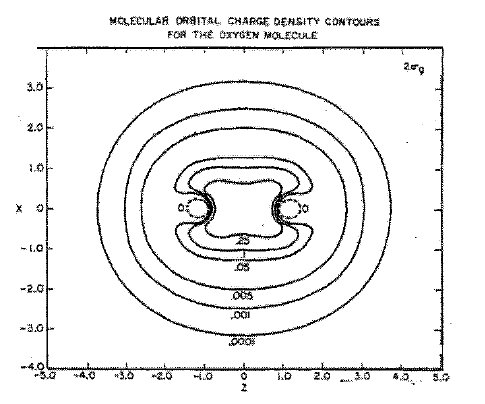
\includegraphics[width=0.6\textwidth]{images/mulliken_figure1.png}
\end{center}

\caption*{Figure 1: [Manual Note for Figures 1-5: As Mulliken says, Figures 1-5 show ``contour maps'' of the molecular orbitals of the oxygen molecule.  Each figure is obtained by solving (or, more accurately, finding an approximate solution to) Schr\"{o}dinger's wave equation for a particular energy level of an electron that would be under the influence of the two oxygen nuclei as well as the other electrons in the $\mathrm{O_2}$ molecule.  Recall from Born that the differential equation for a stationary solution (the $\psi$ ``wave'' for an electron bound to a nucleus) is a function of the momentum operator and the position coordinates.  Therefore, any function $\psi$ that solves this equation will have a value at each coordinate point.  As Mulliken says, the square of that value is proportional to the probability of finding the electron at that point in its orbital.  The contour lines outline regions of probability in each orbital. \vspace{3pt}
\newline  Each figure is one molecular orbital at a particular energy level.  In these figures, the energy level for Figure 2 is higher than in Figure 1, etc., so that Figure 5 is at the highest energy level shown.  The letters and symbols in the upper right corner of each figure give a label to each orbital.  The number is related to Bohr's ``n,'' or quantized energy level.  The Greek letter is connected to the shape of bond formed, and the $g$ or $u$ subscript relates to the mathematical way the two atomic orbitals have been combined to get the molecular orbital.  Notice that the first figure, at the lowest energy level shown, is $2\sigma_g$, and so is at the Bohr energy level of 2.  There is one energy level lower than that, at $n=1$.  This level would correspond to Lewis' ``kernel'' electrons and is not involved in molecular bonding and thus is not included here. \vspace{3pt} 
\newline  Recall from Lewis that oxygen has 6 outer shell electrons.  Mulliken's five orbitals are the orbitals used by the 12 electrons of the oxygen molecule (six on each atom).  There are two electrons in each orbital, with the exception of the $1\pi_u$ orbital (Figure 4).  There are two instances of this orbital, so there are four electrons total in this type of orbital.  Our 12 electrons are therefore found as follows: 2 in $2\sigma_g$ (Figure 1), 2 in $2\sigma_u$ (Figure~2), 2 in $3\sigma_g$ (Figure 3), 4 in $1\pi_u$ (Figure 4), and 2 in $1\pi_g$ (Figure 5).]} 

%\vspace{-10pt}
\end{figure}


\begin{figure}
	\begin{center}
		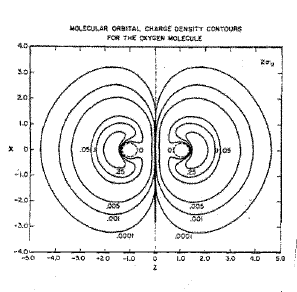
\includegraphics[width=0.6\textwidth]{images/mulliken_figure2.png}
	\end{center}
	% Use the following command to remove the colon from the figure label; Always use it within the environment to keep it local
%%%%	\makeatletter \renewcommand{\fnum@figure}[1]{\figurename~\thefigure} \makeatother
	\caption*{Figure 2}

       % \label{fig:figureX}

%\vspace{-10pt}
\end{figure}


\begin{figure}
	\begin{center}
		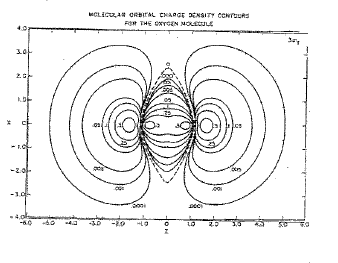
\includegraphics[width=0.6\textwidth]{images/mulliken_figure3.png}
	\end{center}
	% Use the following command to remove the colon from the figure label; Always use it within the environment to keep it local
%%%%	\makeatletter \renewcommand{\fnum@figure}[1]{\figurename~\thefigure} \makeatother
	\caption*{Figure 3}

       % \label{fig:figureX}

%\vspace{-10pt}
\end{figure}

\begin{figure}
	\begin{center}
		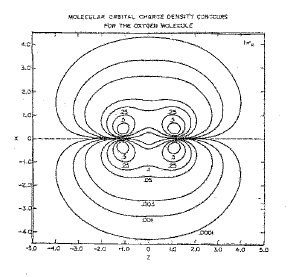
\includegraphics[width=0.6\textwidth]{images/mulliken_figure4.png}
	\end{center}
	% Use the following command to remove the colon from the figure label; Always use it within the environment to keep it local
%%%%	\makeatletter \renewcommand{\fnum@figure}[1]{\figurename~\thefigure} \makeatother
	\caption*{Figure 4}

       % \label{fig:figureX}

%\vspace{-10pt}
\end{figure}


\begin{figure}
\begin{center}
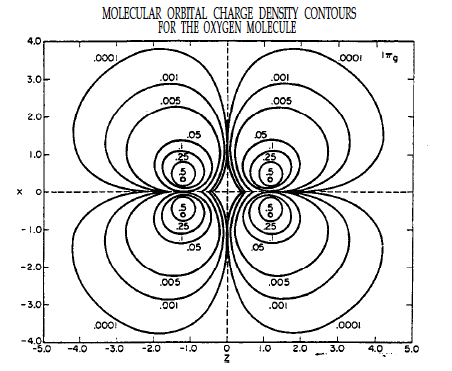
\includegraphics[width=0.6\textwidth]{images/mulliken_figure5.png}
\end{center}
%\captionsetup[figure]{labelsep=none}
\caption*{Figure 5: [Five] Portraits of valence-shell spectroscopic MO's of the oxygen molecule.  Each contour is marked with a number which is the \emph{square} of the value of the MO on that contour.  Each dashed line or curve marks a boundary between positive and negative regions of the MO itself.  From an as yet unpublished paper by P.E. Cade, G.L. Malli and A.C. Wahl; all rights reserved.}
%\vspace{-10pt}
\end{figure}


Figures 1-5 show contour maps of the true accurate valence-shell MO's of the oxygen molecule, as obtained by calculations at the Laboratory of Molecular Structure and Spectra at the University of Chicago.  In these ''portraits'' of MO's, each contour is marked with a number which gives the magnitude, not of the MO itself, but of its square.  This use of the square is particularly instructive because the square of the value of the orbital at any point in space is proportional to the probability of finding the electron at that point when it is in that orbital.  Thus what Figures 1-5 show are really probability density portraits, rather than direct pictures of the MO's.  Additional portraits of this kind, and helpful discussion of them, are contained in two recent articles.\footnote{A.C. Wahl, \emph{Science}, 151 (1966) 961; W.M. Huo, \emph{J. Chem. Phys.}, 43 (1965) 624.}  The necessary calculations which are making MO portraits possible are extremely complex and require the use of large computing machines.  They have involved the work of a number of people, of whom I shall speak later.

A definite \emph{energy} is associated with each orbital; either atomic or molecular.  The best interpretation of this orbital energy is that it is the energy required to take the electron entirely out of the orbital, out into free space.  The lowest-energy orbitals are those which favor regions of space closest to the nucleus, in the case of atomic orbitals, or closest to one or more nuclei in the case of molecular orbitals.

In what I like to call the \emph{normal state}, but most people call the ground state (German ''Grundzustand''), of an atom or molecule, the electrons are settled in the lowest-energy orbitals that are available.  (Bohr called it the ''permanent'' state.)  Higher in energy than the normal-state orbitals and favoring regions of space farther from the nucleus or nuclei, there are great numbers of \emph{vacant} orbitals, into any one of which, however, any electron can go if given enough extra energy, by the right kind of a push or kick.  These ordinarily vacant AO's or MO's are called excited orbitals, and when one (or sometimes more) electrons of an atom or molecule have been kicked into excited orbitals, the atom or molecule is said to be \emph{excited}.  Excited states of atoms or molecules, with some exceptions, do not last long.  Instead, the molecule loses its extra energy, generally either in collisions with other molecules, or by sending it out in the form of electromagnetic radiation: that is, visible or infrared or ultra-violet light or X-rays.  A careful study of the spectrum of wave lengths of such radiation gives important information about the forms and energies of the orbitals involved, and about other properties of the atom or molecule both in its normal and in various excited conditions.  

A prominent feature of Bohr's 1922 theory of atoms was the Aufbauprinzip (build\-ing-up principle) according to which if electrons are fed one by one to an atomic nucleus and the atom is allowed to subside into its normal state, the first electrons fall into the lowest-energy orbits, the next into those next lowest in energy, and so on.  In this way Bohr first explained the formation of successive electronic shells and the periodic system of the chemical elements.  In the modern quantum mechanics, exactly the same description holds good except that atomic orbitals replace orbits.  In the \emph{molecular orbital method} of describing the structure of molecules, an entirely analogous use is made of an Aufbauprinzip in which electrons are fed into molecular orbitals.

However, there is also another way of describing molecules, usually called the valence-bond method.  This was initiated by the work of Heitler and London on the hydrogen molecule, and developed further by Slater and Pauling especially.  In this method, each molecule is thought of as composed of atoms, and the electronic structure is described using atomic orbitals of these atoms.  This approach, which I prefer to call the \emph{atomic orbital method},\footnote{To speak of the ''valence-bond method'' places the emphasis in chemical bonding on a few pairs of electrons holding atoms together in the Heitler-London manner, whereas actually the interactions of many of the other electrons often have very important effect on the stability of molecules.} is a valid alternative to the MO method, which in its most general form regards each molecule as a self-sufficient unit and \emph{not} as a mere composite of atoms.

The AO method at first appealed to chemists because it was much easier to fit into customary ways of thinking.  However, it has become increasingly evident that the MO method is more useful for a detailed understanding of the electronic structures of molecules, especially if extensive theoretical calculations are to be made, as is not increasingly feasible with the help of modern large-scale digital computers.  Also the MO method is far better suited for an understanding of the \emph{electronic spectra} of molecules and thus also of their photochemical behavior, a subject which is now receiving increasing (and increasingly understanding) attention.

I have just stated that the AO and MO methods are valid alternatives to each other, although they differ with respect to ease of understanding and of application.  But why is not one right and the other wrong?  The explanation is, roughly, that both methods correspond only to \emph{approximate} solutions of the \emph{complete} equations which govern the behavior of molecules that contain more than one electron.  Starting from either method, further and in general very difficult calculations are needed for an exact understanding.

Why this is true can be seen in comparing an atom with a planetary system.  In a planetary system, the sun is vastly larger than any of the planets and the gravitational attractive force it exerts on each planet is exceedingly large compared with the small gravitational forces which the planets exert on one another.  Thus the motion of each planet in its orbit can be calculated to a satisfactory degree of exactness by a method called \emph{perturbation theory}.  However, it has not proved mathematically possible to obtain an absolutely exact solution which would be true over very long intervals of time.  The same statement holds for every situation in which more than two objects are exerting forces on another.  Such a situation is called a many-body problem.

Although with a sun and planets the lack of a solution of the many-body problem is not very serious, matters are very different for an atomic nucleus and its electrons, for two reasons: (1) the electrons in an atom, though not really close together, are vastly more crowded than planets in a planetary system; (2) the forces between electrons, though not as large as the force exerted by the nucleus on each electron, are nevertheless too large to be treated as small perturbations as could be done for planets and a sun.  These difficulties existed in the old quantum theory of electron \emph{orbits}, and similar difficulties still occur for \emph{orbitals} in the modern quantum mechanics.  Perturbation theory is valuable in both the Bohr theory and in quantum mechanics, but it does not easily solve the many-body problem.  Consequently, it is an exceedingly difficult matter to obtain a reasonably exact understanding of the electronic structure of atoms or, especially, of molecules, except if there is only one electron, as in the hydrogen atom, or (more difficult) in the positively charged hydrogen molecule ion.  In these cases, the AO (for H) or the MO (for $\mathrm{H_2^+}$) is an exact solution of Schr\"{o}dinger's equation.  The first fairly exact calculation on the normal state of $\mathrm{H_2^+}$, by Burrau,\footnote{O. Burrau, \emph{Kgl. Danske Videnskab. Selskab}, 7 (1927) 1.} is the earliest example of the nearly exact calculation of the form of a true MO.

Thus we are brought face to face with the fact that when the structure of a typical atom or molecule is described by assigning each electron to an orbit, this description is usually rather far from being exact.  It is good enough to be extremely useful, and in the case of atoms is sufficient to account for the main features of atomic structure, the periodic system of the elements, and atomic spectra, but it is by no means exact.  Analogous comments apply for the description of the structure of a molecule in terms of electrons assigned to MO's.

The description in terms of a single set of orbitals for the electrons is called an \emph{independent-particle model}.  It is a kind of model which is very nearly exact in the case of the orbits of planets going around a sun, but is only a rather rough approximation in the much more crowded situation, with much stronger forces, of electrons in an atom or molecule.  What is lacking is called \emph{electron correlation}.  Because orbitals are based on an allowance only for the \emph{average} forces exerted by other electrons, the simple orbital description needs to be rather strongly corrected for the fact that electrons in their motions are sometimes closer, sometimes less close than their average distance, so that the forces between them vary accordingly, and to an important extent.

Now let us return to the question of how it is possible that both of two seemingly very different methods, the AO and the MO method, can represent useful descriptions of the electronic structures of molecules in their normal states and can help us to understand chemical bonding.  The answer lies in the fact that both methods need a considerable amount of correction for electron correlation before their descriptions become accurate.  The fact that they differ so strongly from each other is explained by noting that they lie as it were on \emph{opposite sides} of an accurate description, which then lies between them.  For a full explanation, however, much more must be said than is possible here.  Nevertheless, it seems to be true that the MO method is better suited not only as a basis for rather accurate calculations at the degree of approximation possible in an independent-particle method, but also that it is well suited to going further with the necessary corrections to take electron correlation rather well into account.\footnote{For some simple diatomic examples, see G. Das and A.C. Wahl, \emph{J. Chem. Phy.}, 44 (1966) 87.}

Now before going further, I would like to return briefly to the historical development of MO ideas in the early 1920's before the time of the modern quantum mechanics.  Although Bohr in his early papers' proposed molecular models in which pairs of electrons rotating in a circular orbit between two atoms served to form a chemical bond, later calculations based on this model, even for the simplest case of the hydrogen molecule, proved as \emph{unsuccessful} as the Bohr theory of the hydrogen atom has proved successful.

On the other hand, molecular spectroscopists in the early 1920's found that the excited electronic states of diatomic molecules show various features which could be explained by postulating resemblances to those of atoms.\footnote{Details and references are given in an article entitled ''Molecular Scientists and Molecular Science: Some Reminiscences'', \emph{J. Chem. Phys.}, 43 (1965) S2-11.  [Also], see the introduction to ''Report on Molecular Orbital Theory'', \emph{J. Chem. Phys.}, 46 (1949) 497, and references given there.}  This experimental evidence suggested that the electrons in molecules, to an extent similar to that of electrons in atoms, are moving in something like orbits and that some sort of Aufbauprinzip is valid for the electronic structures of molecules.

My own work in 1923-25 was at first concentrated on trying to understand the visible and ultraviolet spectra of diatomic molecules, called band spectra, at the Jefferson Physical Laboratory of Harvard University.  In learning about this field, which at that time was completely new to me, I had the very kind help of Professor F. A. Saunders in experimental spectroscopy, and Professor E. C. Kemble in quantum theory.  I also benefited greatly from correspondence with Professor R. T. Birge of the University of California.  It is very interesting at this point to note that in those days basic spectroscopy and the theory of molecular electronic structure were being studied primarily by physicists (my papers until the advent of the \emph{Journal of Chemical Physics} were published in the \emph{Physical Review} or the \emph{Reviews of Modern Physics}).  Now, however, these subjects, as well as the newer branches of spectroscopy (nmr, esr, etc.) which were born in physics laboratories, are generally considered to belong primarily to chemistry.  These circumstances account for the fact that, although my B. S. and Ph.D. degrees were in chemistry, I have for a long time been a member of physics departments, where I am classified as a molecular physicist.  Only rather recently have I become formally associated also with chemistry departments, thereby giving recognition to the migration of molecular spectroscopy and MO's from physics toward chemistry.  Nevertheless, the basic facts of these areas of science do still lie in the border region between physics and chemistry.

Now to return to my early efforts to understand diatomic band spectra: the detailed structures of these spectra fell into several distinct types which indicated the existence of several types of molecular electronic states.  Moreover, these types appeared to differ, as did the atomic states of Bohr-Sommerfeld theory, in respect to angular momentum properties.\footnote{The major structural features of diatomic spectra are dominated by the existence of molecular vibrations and rotations, but the detailed structures depend on the interaction of molecular rotation with electronic orbital and spin angular momenta.} Following a suggestion of Birge, I called them S, P, D states, using the same symbols as for atomic states, although the characteristic described by the symbol was not total orbital angular momentum as in the case of the atomic symbol, but only the axial component of angular momentum.

With the advent of quantum mechanics about 1926, the short-comings of the old quantum theory of atoms and its inability to deal seriously with molecules were quickly removed.  Among other changes, atomic electron orbits were replaced by atomic orbitals, although the \emph{name} orbital was given only later, in 1932.  My friend Friedrich Hund, whom I first met in G\"{o}ttingen in 1925, and with whom I had many discussions then and in 1927 and later, applied quantum mechanics to a detailed understanding of atoms and their spectra, and then to the spectra and structure of molecules.\footnote{Details and references are given in an article entitled ''Molecular Scientists and Molecular Science: Some Reminiscences'', \emph{J. Chem. Phys.}, 43 (1965) S2-11.}  Using quantum mechanics, he quickly clarified our understanding of diatomic molecular spectra, as well as important aspects of the relations between atoms and molecules, and of chemical bonding.  It was Hund who in 1928 proposed the now familiar Greek symbols $\Sigma$, $\Pi$, $\Delta$, for the diatomic molecular electronic states which I had been calling S, P, and D.  Molecular orbitals also began to appear in a fairly clear light as suitable homes for electrons in molecules in the same way as atomic orbitals for electrons in atoms.  MO theory has long been known as the Hund-Mulliken theory in recognition of the major contribution of Professor Hund in its early development.

I have emphasized already that a \emph{true} AO or MO is properly considered as one which is appropriate for an electron assumed under the influence of the \emph{average} electric field of the other electrons, all in accurate self-consistent-field orbitals.  However, for MO's there are also several very useful approximations to the exact method.  These approximations can be briefly characterized as corresponding to varying degrees of localization or \emph{delocalization}.  The purest and most accurate MO method, yielding true MO's, involves the maximum amount of delocalization, with every MO spread to some extent\footnote{To be sure, often some (or even most) of them turn out to be mainly (or, in some cases, almost wholly) concentrated near particular atoms or groups of atoms.} over the whole molecule.  These pure MO's I like to call \emph{spectroscopic MO's}, since it is they which are particularly important for understanding electronic spectra in molecules.  They are also of especial importance for understanding ionization processes; each of the simplest ionization processes corresponds to removal of an electron from a particular spectroscopic MO.  

Several types of more or less localized MO methods, although they represent somewhat less accurate descriptions, are also useful, especially in understanding and describing chemical bonding.  On starting with a localized-MO description, and afterward proceeding to one or more successive steps of delocalization, and then finally introducing electron correlation, we can often gain much added insight by this step-wise approach into the chemical consequences of what the electrons are doing.  The most fully localized sets of MO's include bond MO's localized between two or sometimes three or four atoms, taken together with some MO's so strongly localized that they are just AO's (but often \emph{hybrid} AO's) on single atoms; we note there that, after all, an AO can be considered as a special type, the simplest possible type of MO.  These localized MO's I like to call \emph{chemical} MO's (or just \emph{chemical orbitals} because of the fact that some of the orbitals used are now really AO's).  In simple molecules, electrons in chemical MO's usually represent the closest possible quantum-mechanical counterpart to G. N. Lewis' beautiful pre-quantum valence theory with its bonding electron pairs, lone pairs, and inner shells.  It is the inner-shell and the lone-pair electrons which are in AO's when chemical MO's are used.

It was Hund in a paper on chemical bonding\footnote{F. Hund, \emph{Z. Physik.}, 73 (1931) 1.} who first referred to $\sigma$ and $\pi$ bonds: a single bond is a $\sigma$ bond, a double bond is a $\sigma$ plus one $\pi$ bond,\footnote{According to their original definition, valid for diatomic (or linear) molecules, $\pi$ orbitals are two-fold degenerate.  That is, there are two varieties of $\pi$ orbitals which differ only by a $90^{\circ}$ rotation around an axis of cylindrical symmetry.  But in the case of double bonds, only one of these is used and the other no longer exists as such but is mixed with $\sigma$ orbitals.  The $\pi$ orbitals of double bonds really ought to have a different name.} a triple bond is a $\sigma$ plus two $\pi$ bonds, and each bond corresponds to a pair of electrons in a bond MO localized around the two atoms of the bond.  While, as I have already said, it is necessary for a thorough understanding to take the effects of all the electrons into account, a consideration just of electrons assigned to localized bond MO's does give a useful approximate understanding of important aspects of chemical bonding, for example, the existence of nearly free rotation around single bonds but restriction of the bonded and neighboring atoms to a plane in the case of double bonds.

\begin{figure}
\begin{center}
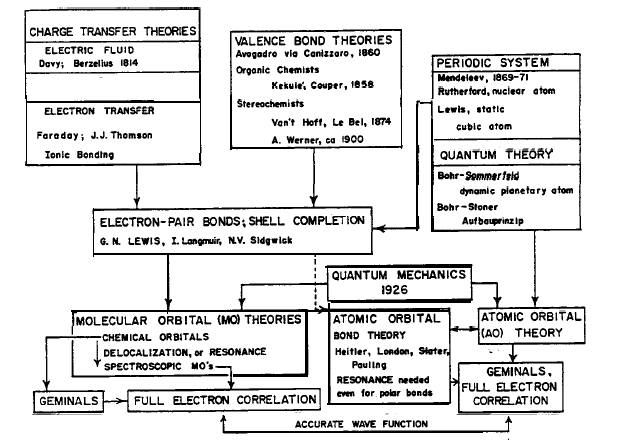
\includegraphics[width=0.7\textwidth]{images/mulliken_figure6.png}
\end{center}
%\captionsetup[figure]{labelsep=none}
\caption*{Figure 6: Historical flow diagram of ideas leading to MO and AO theories of molecular electronic structure, and on to accurate wave functions.  From the author's 1965 Silliman Lectures at Yale University}
%\vspace{-10pt}
\end{figure}


Before going further, I should like to show four slides\footnote{These slides have been borrowed from my 1965 Silliman lectures at Yale.} to illustrate the relation of G. N. Lewis' theory to MO theory using chemical orbitals, and also to summarized some other historical relationships.  Figure 6 is more or less self explanatory.  It is designed to show, first of all, how Lewis resolved the long-standing conflict between, on the one hand, ionic and charge-transfer theories of chemical bonding and, on the other hand, the kind of bonding which is in evidence in bonds between equal atoms, for example, in $\mathrm{H_2}$ or $\mathrm{C-C}$ in $\mathrm{C_2H_6}$: Lewis represented each bond by a pair of electrons placed between the two bonded atoms, with the electron pair located closer to one atom than to the other in the case of polar bonds.  Figures 7 and 8 show some examples of Lewis structures, including example of coordination compounds like $\mathrm{H_3N \cdot BH_3}$, (as pointed out later by Sidgwick) $\mathrm{CO \cdot (NH_3)_6^{+3}}$.  In coordination compounds, Lewis lone pairs belonging to electron-donor molecules, for example $\mathrm{NH_3}$, are shared to some extent with electron-deficient molecules or ions like $\mathrm{BH_3}$ or $\mathrm{CO^{3+}}$, forming ''dative bonds'' or partial dative bonds.

%Consider inserting figures 6, 7, and 8, probably redrawing them.

\begin{figure}
\begin{center}
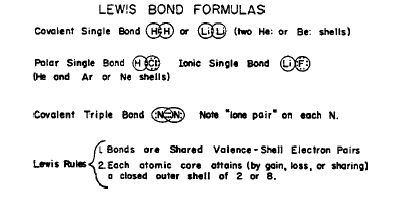
\includegraphics[width=0.6\textwidth]{images/mulliken_figure7.png}
\end{center}
%\captionsetup[figure]{labelsep=none}
\caption*{Figure 7: (Caption for both Figures 7 and 8.) Examples of G.N. Lewis bond formulas, showing also pair or octet completion by sharing.  From the author's 1965 Silliman Lectures at Yale University.}
%\vspace{-10pt}
\end{figure}

\begin{figure}
\begin{center}
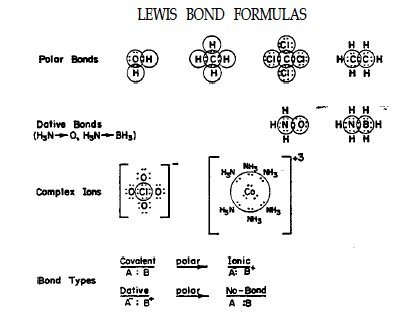
\includegraphics[width=0.6\textwidth]{images/mulliken_figure8.png}
\end{center}
%\captionsetup[figure]{labelsep=none}
\caption*{Figure 8: [See caption for Figure 7.]}
%\vspace{-10pt}
\end{figure}

Lewis made use of an Aufbauprinzip in terms of electron shells (paris and octets mainly) which could in part be obtained by \emph{sharing}, so that the same pair of electrons could be counted in the shells of both of two atoms, as suggested by circles in Figures 7 and 8 (not shown in every case).  For individual atoms, Lewis' electron shells were three-dimensional, in contrast to Bohr's planar electron orbits, in this respect being closer to the present quantum mechanics than the Bohr theory.  However, of course Lewis' theory was empirical, schematic, and purely qualitative, and gave no explanation of how the electrons might be moving or why and how they should station themselves between atoms to form bonds, or in pairs or octet in shells.  Bohr's early papers included some pictures of pairs of electrons (the electrons of each pair moving on opposite sides of a single circular circular orbit) forming chemical bonds between atoms, for example in $\mathrm{H_2}$ and in $\mathrm{CH_4}$ in three-dimensional arrangements.

The Heitler-London AO theory of the chemical bond is rather generally regarded as the quantum-mechanical counterpart of Lewis' electron-pair bond.  However, a pair of electrons in a bond MO represent an approximately equally good counterpart in the case of a symmetrical (homopolar) bond, while for a polar bond (as in HCl or in $\mathrm{H_2O}$) they represent a much better counterpart.

The justification for this last statement can be seen most easily by writing the \emph{bond} MO in the LCAO approximate from $\alpha \chi _a + \beta \chi _b $, where $x_a$ and $x_b$ are AO's of atoms $a$ and $b$.  For homopolar bonds, $a = \alpha$, but for polar bonds $\alpha$ and $\beta$ are unequal to an extent which matches the polarity of the bond, for example, $\alpha < \beta$ for an HCl or NaCl molecule, if atom $\alpha$ is H or Na, with a much greater inequality for NaCl than for HCl.  (Pure ionic NaCl would be represented by $\alpha = 0, \; \beta = 1$), but actually the NaCl molecule is not quite pure ionic, or if one wants to call it pure ionic, it is necessary to say also that the Cl-ion is strongly polarized.)  Thus the chemical-MO theory has the same flexibility as the Lewis theory in representing polar bonds, while the AO theory has to assume mixtures of Heitler-London and ionic bonding to represent polar bonds.  The chemical-MO theory also furnishes the counterpart of Lewis' lone pairs ($\mathrm{NH_3}$ is a good example), and also shows they can be modified into pairs occupying polar bond MO's in coordination compounds.  

Figure 6, after illustrating Lewis' synthesis of earlier ideas, goes on to show how the intervention of quantum mechanics in 1926 permitted further progress by MO theories, and then indicates the necessity of the final step of electron correlation for accurate descriptions.  It also shows the alternative route \emph{via} AO theories of atoms and AO bond theory, followed by electron correlation again as a final step to give accurate wave functions identical in content, if not necessarily in form, with those obtained \emph{via} MO theory.

\begin{figure}
\begin{center}
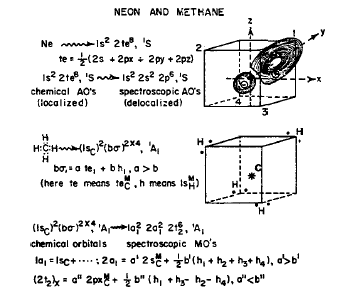
\includegraphics[width=0.6\textwidth]{images/mulliken_figure9.png}
\end{center}
%\captionsetup[figure]{labelsep=none}
\caption*{Figure 9: Chemical and spectroscopic MO's, illustrated by the neon atom and the methane molecule.  From the author's 1965 Silliman lectures at Yale University.}
%\vspace{-10pt}
\end{figure}


Figure 9 illustrates for the $\mathrm{CH_4}$ molecule how chemical MO's and spectroscopic MO's are related, and shows also how chemical MO's could be used instead of spectroscopic MO's for an atom like neon.  The figure depicts for the neon atom just one of four localized or chemical AO's which are identical except for their orientation; each one is symmetrical about a line directed toward one of the four corners of a tetrahedron, marked 1, 2, 3, and 4.  The four BMO's (bond MO's) of $\mathrm{CH_4}$ if they were depicted (instead a pair of dots as in a Lewis formula is shown for each) would be similar in appearance to the chemical AO's of neon except that each one would spread out somewhat more around its appropriate H nucleus.  LCMAO expressions (the extra M means \emph{modified} - see discussion near the end of this paper) are given for these BMO's, and also for the spectroscopic MO's of $\mathrm{CH_4}$.

Next I must mention the simple LCAO (linear combination of AO's) procedure which for many years represented the usual way of trying to approximate the forms of MO's, whether of localized or delocalized type.\footnote{See the introduction to ''Report on Molecular Orbital Theory'', \emph{J. Chem. Phys.}, 46 (1949) 497, and references given there.} For metals, Bloch in 1928 used fully delocalized MO's extending throughout the metal, constructed approximately as linear combinations of valence-electron AO's of all the atoms.  Lennard-Jones in 1929 pointed out the general usefulness of simple LCAO expressions in approximating valence-shell diatomic MO's; for inner shells he used AO's.\footnote{Perhaps the first example of the LCAO type of description was its use by Pauling for $\mathrm{H_2^+}$, - which, however, can be considered as an example of the AO equally as well as of the MO method.}  Herzberg then emphasized that the number of bonds in a diatomic molecule can be set equal to half the difference between the number of electrons in bonding MO's (which have \emph{additive} LCAO forms, that is $\alpha$ and $\beta$ of the same sign in $\alpha \chi _a + \beta \chi _b $) and the number in \emph{antibonding} MO's (which have \emph{subtractive} LCAO forms, that is $\alpha$ and $\beta$ of opposite signs).  H\"{u}ckel developed his very simple LCAO treatment for the $\pi$ electrons in unsaturated and organic molecules, a procedure which while rough and subject to some serious limitations, has been very useful to the organic chemists for many years.  Before they became much interested, however, the subject had been developed further by Coulson, Longuet-Higgins, Dewar, and others, and presented rather forcefully to them by Dewar.

I must not take too long for matters of historical interest, since I want to say something about current developments and about the future, so I will now give only a condensed account of some of the further developments of MO theory.

I have already mentioned the use of the LCAO method for the rather roughly approximate visualization of MO's of diatomic molecules and of metals, and also (although until recently for $n$ electrons only) for many of the important molecules of organic chemistry.  In the years 1932-1935 I turned my attention to the exciting possibilities of understanding the electronic structures and spectra of many small polyatomic molecules, many of them prototypes of larger organic and inorganic molecules.  In so doing, I used molecular symmetry properties and the LCAO method.  At that time J. H. van Vleck called my attention to the applicability of Bethe's group-theoretical determination of the irreducible representations for the orbitals of an atom in a crystal to the classification of MO's.  For the different species of MO's I then adopted a system of symbols nearly like that in a paper on Raman spectra by Placzek of which I secured a proof copy.\footnote{"On the Classification of Molecular States", see \emph{J. Chem. Phys.}, 23 (1955) 1997-2011.}  A particularly appealing type of molecules for understanding by the MO method was that of the complex ions of high symmetry, but after a brief mention, I postponed going into these, saving them as a choice tidbit for some future occasion which, however, got indefinitely postponed.  In recent years others have done full justice to this subject of ligand-field MO theory.

Among later aspects of my own work was an interest in the absolute intensities of molecular spectra, in particular intramolecular charge-transfer spectra.  Growing out of that were some ideas on conjugation and hyper-conjugation in organic-chemical molecules.  Later on, in trying to explain some new spectra of iodine in solutions in benzene or other related compounds, I became interested in the interaction of molecules with one another involving the partial transfer of an electron from a donor to an acceptor molecule to form a molecular complex.  In this connection I got into a study of intermolecular charge e-transfer spectra, of which the benzene iodine spectrum of Benesi and Hildebrand is the classic example.

I mention all these things together because they are all concerned with what happens to our understanding of molecules when less and less localized approximate MO's are used.  I have said earlier that the best or truest MO's are those which are \emph{fully} delocalized.  However, it is very instructive to start with localized MO's, and see what we can learn at each step as the theoretical description is made more accurate in successive steps of delocalization.  Consider for example the 1,3-butadiene molecule.  The simplest set of chemical orbitals would here consist of a K shell (IS) MO on each of the four carbon atoms, six $\sigma$-bond MO's for carbon-hydrogen bonds, three carbon carbon $\sigma$-bond MO's and two carbon-carbon p-bond MO's corresponding to the chemical formula [below:]



%insert diagram 9a
% this framing is wonky and breaks easily
\begin{wrapfigure}[6]{r}{0.5\textwidth}
	\vspace{-20pt}
	\begin{center}
	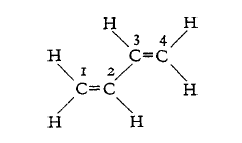
\includegraphics[width=0.3\textwidth]{images/mulliken_figure9a.png}
    \end{center}
    \vspace{-10pt}
\end{wrapfigure}

The $\pi$-electron part of the electron configuration would then consist in two pairs of electrons occupying two bond MO's 

\begin{equation*}
\varnothing _{12} = \alpha (\chi_1 + \chi_2) \;\; \varnothing _{34} = \alpha (\chi_3 + \chi_4)
\end{equation*}

\noindent where the four $\chi$'s are $\pi$ AO's on atoms 1, 2, 3, and 4 of the chemical formula.  The pair in the MO $\varnothing _{12}$ forms a $\pi$ bond between atoms 1 and 2, that in $\varnothing _{34}$ forms an exactly similar bond between atoms 3 and 4.


However, a distinctly improved approximate wave function\footnote{R.S. Mulliken, \emph{J. Phys. Chem.}, 66 (1962) 2306.} is obtained if the two localized p-bond MO's $\varnothing _{12}$ and $\varnothing _{34}$ are replaced by two new fully delocalized MO's (spectroscopic $\pi$ MO's) as follows, each extending over all four atoms:

\[\varnothing_I = b\chi_1 + c\chi_2 + c\chi_3 + b\chi_4 \]
\[\varnothing_{II} = b ^\prime \chi_1 + c ^\prime \chi_2 - c ^\prime \chi_3 - b ^\prime \chi_4 \]


\noindent with $c$ somewhat larger than $b$ and $c^\prime$ smaller than $b^\prime$ (b, c, $b^\prime$, $c^\prime$ all positive).  Both $\varnothing_I$ and $\varnothing_{II}$ given bonding between atoms 1 and 2, and between 3 and 4, so that the total $\pi$ bonding in the original bonds is not much changed, but now the electrons in $\varnothing_I$ give $\pi$ bonding between atoms 2 and 3, while those in $\varnothing_{II}$ given antibonding between 2 and 3, but because $c>b$ and $b^\prime < c^\prime$, the net bonding effect of the pair of electrons in $\varnothing_I$ outweighs the antibonding effect of those in $\varnothing_{II}$, giving some net $\pi$ bonding between atoms 2 and 3.  Without delocalization, then electron pairs in $\varnothing_{12}$ and $\varnothing_{34}$ would have created a net antibonding effect\footnote{R.S. Mulliken, \emph{J. Phy. Chem.}, 66 (1962) 2306} (repulsion) between atoms 2 and 3. 


Delocalization here results in a small decrease in the calculated energy but, more important, it accounts for the stability of the arrangement of the atoms in one plane, and predicts certain differences in chemical properties as compared with those which would be expected if there were no delocalization.  When two double bonds are separated by one single bond, as in butadiene, the double bonds are called conjugated.  Conjugated $\pi$-electron molecules are characterized by special properties which are understandable by MO theory in terms of $\pi$-electron delocalization, as just described.  Of course the \emph{actual} molecule shows those properties which correspond to conjugation or $\pi$ delocalization; the localized description is an approximation which much less accurately describes the character of the actual molecule.


Finally, in a completely delocalized description the various localized MO's are replaced by spectroscopic MO's, which are fully delocalized $\sigma$ MO's of various symmetry types extending over the whole molecule.  This final stage of delocalization can be categorized as as variety of hyperconjugation, although not one of the most typical or important kinds.

In the 30's I tried to deduce all I could about MO's from qualitative considerations of energy and symmetry taken together with empirical evidence from molecular spectra and other properties.  During this period and up to the time of the war in the early 40's, molecular spectroscopy was a major activity in our laboratory, under the able guidance in particular of Dr. Hans Beutler and then of Dr. Stanislaus Mrozowski.  Toward the end of this period the enthusiastic assistance of Mrs. C. A. Rieke made possible many desk-machine calculations on hyperconjugation and on $\pi$-electron systems using the H\"{u}ckel method until then everyone was neglecting because they made the calculations more complicated.  After the war I took up this matter again, and wrote about various relations of overlap integrals to chemical bonding.  I began also to be very dissatisfied with other inadequacies of H\"{u}ckel-method calculations.\footnote{See the introduction to ''Report on Molecular Orbital Theory,'' \emph{J. Chem. Phys.}, 46 (1949) 497, and references given there.}

C. C. J. Roothaan had come to me as a graduate student in physics in 1947, already so well prepared in his studies with R. L. Kronig at Delft that I could only make some suggestions to him about problems on which calculations would be interesting.  One study that he made by the H\"{u}ckel method dealt with the structure of the ethylene molecule and its exited states and their behavior on twisting the molecule.  The theoretical calculation confirmed the qualitative conclusion that twisted ethylene is strongly stabilized by hyperconjugation.

I tried to induce Roothaan to do his Ph.D. thesis on H\"{u}ckel-type calculations on substituted benzenes.  But after carrying out some very good calculations on these he revolted against the H\"{u}ckel method, threw his excellent calculations out the window, and for his thesis developed entirely independently his now well known all-electron LCAO SCF self-consistent-field method for the calculation of atomic and molecular wave functions, now appropriately referred to, I believe, as the Hartree-Fock-Roothaan method.  After a short period at Catholic University, Roothaan returned to our laboratory, where he expressed an unquenchable ambition to conquer the calculation of some of what then seemed almost incredibly difficult electron-repulsion integrals, and which had been one of the main obstacles to converting the molecular-orbital theory from a descriptive and semi-empirical to a more nearly quantitative theory.  Another very important contributor to this endeavor at that time was Klaus Ruedenberg, who since then has added very much to our insights into the nature of chemical bonding.

I shall return shortly to the theme of the purely theoretical calculation of molecular structures and properties, but first wish to mention another development which has been very fruitful.  Robert Parr spent the summer of 1949 at Chicago, and together we worked out some interesting applications of the semi-empirical $\pi$-electron - only LCAO SCF method (pioneered by Goeppert-Mayer and Sklar in 1939) for $\pi$-electron organic molecules.  Somewhat later Parr and his student Pariser developed the Pariser-Parr method to deal with $pi$-electron molecules in a way which (along with the rather similar Pople method) represented a great imporvement for an improved understanding of molecules of importance in organic chemistry and biology.

In the late 40's it was not yet clear that really accurate theoretical calculations on molecules would be feasible, and we were happy to make progress by semi-empirical methods.\footnote{R.S. Mulliken, \emph{Chem. Rev.}, 41 (1947) 201.}   We did not realize that the big modern digital computers would become available and be rapidly improved in size and flexibility, and would transform theoretical computations into a tool which has already begun to compete with or in some cases even to go beyond experimental work in the laboratory.  The rest of my speech will be devoted to some of the progress which has already been made in that direction.

What I shall now present to you will not be my own work, but that of those who have been my associates in our group at Chicago.  Let me also say that it is only because of lack of time that I shall say very little about the many others at other institutions in various countries who have also made major contributions; I hope they will forgive me for this omission.

Here let me quote briefly, with minor changes, from a 1958 paper\footnote{R.S. Mulliken and C.C.J. Roothaan, ''Broken Bottlenecks and the Future of Molecular Quantum Mechanics,'' \emph{Proc. Natl. Acad. Sci. (U.S.)}, 45 (1959) 394-398.} which is already out of date because of the rapid development of bigger and better computers.

''Dirac once stated that, in principle, the whole of chemistry is implicit in the laws of quantum mechanics, but that in practice, prohibitive mathematical difficulties stood in the way \ldots ''

''In the early days of quantum mechanics, many of the world's best theoretical physicists engaged in calculations on molecules using the then new tool of quantum mechanics, in the hope of understanding and explaining molecular properties.  But except in the simplest cases, those of the helium atom and the hydrogen molecule, the computations proved to be complicated and laborious without yielding more than roughly approximate results.  Frustrated and repelled, many of the theorists turned to other problems.''

''Perhaps the most forbidding difficulty was that of the evaluation and numerical computation of certain integrals representing the energies of repulsion between electrons in different orbitals.  After the early years of quantum mechanics, the work of a number of Japanese, English, American, and other investigators was directed toward breaking the bottleneck of the difficult integrals but it was only in the 50's that really substantial progress was made.  Among the most active workers were Kotani and his group in Japan, Boys in Cambridge, Coulson and his group at Oxford, L\"{o}wdin and his group in Uppsala, Slater's group at M.I.T. and our own group at Chicago.''

''A major and indeed crucial step beyond the development of formulas for molecular integrals was the programming for large electronic digital computers of the otherwise still excessively time-consuming numerical computation of these integrals, and of their combination to obtain the desired molecular wave functions and related molecular properties.  The pioneering work in this field was that of C.F. Boys at Cambridge, England.''

Now let me turn to the work at Chicago in the area of large-scale machine computations, for which my colleague Roothaan has been primarily responsible with his students and co-workers.  This work has gone through successive stages of development with increasingly powerful machines.  The calculations to which I shall refer are so-called non-empirical, in other words, purely theoretical, calculations in which all the electrons in the atom or molecule are included, as contrasted with the still extremely valuable semi-empirical methods already mentioned which took specific account only of the $\pi$-valence electrons.  A major improvement in depth of understanding is added when all the electrons, inner shell as well as outer shell, $\sigma$ as well as $\pi$, are included in the calculation.

The first all-electron calculation at Chicago was done by C. W. Scherr for his Ph.D. thesis published in 1955; it was a Roothaan-type LCAO SCF calculation on the nitrogen molecule using, however, only what might be called a skeleton crew of AO's in his LCAO expressions, a so-called \emph{minimal basis set}.  This calculation done by Scherr on desk computers with the help of two assistants took him two years.  The same computation could now be repeated in about two minutes with the largest computers now available, provided of course that the preliminary work of writing the machine program had been done.

Writing a good machine program for molecular electronic structure calculations is, however, a very difficult and time-consuming operation.  Two generations of machine programs have been developed at Chicago under Roothaan's direction, and a third is now being prepared.

Extensive computations have been made using the first two of these programs for diatomic molecules, especially by Dr. B. J. Ransil and associates with the first program, and by Dr. Paul E. Cade, Dr. Winifred M. Huo, and Dr. A. C. Wahl and associates with the second program, for whose preparation Wahl, Huo and others were largely responsible.  There were also machine programs and very extensive computations for \emph{atoms}.

In the second machine program, provision was made for building up the MO's from a \emph{large number} of Slater-type orbitals, or better stated (as proposed by Roothaan and others), Slater-type \emph{functions} (STF's).  This LC STF approach represent the use of the Roothaan method in its general form to build up MO's.

LCAO calculations until recently have for the most part been minimal-basis-set calculations, in which the number of AO's used in constructing MO's has been equal to the number of occupied AO's of the atoms from which the molecule can be formed, or at most includes one more valence-shell AO per atom.  For example, the minimal basis set for LCAO MO's of $\mathrm{Li_2}$, of 1s and 2s AO's, just as in the Li atoms, \emph{plus} a $2p\sigma$ AO, which is not used in the free atom in its normal state.  Inclusions of the $2p\sigma$ AO permits $2s-2p\sigma$ hybridization, which is important if reasonably good LCAO MO's are to be obtained.  For $\mathrm{N_2}$, the minimal basis set consists of $1s$, $2s$, $2p\sigma$, and $2p\pi$ AO's for each atom, all of which are occupied in the normal state of the free atom.  In the earlier calculations, each AO in an LCAO MO expression was approximated by a single Slater AO (which is an STF of a size governed by certain very useful simple empirical rules which Slater set down in 1930).\footnote{For a review of Slater's work, see R.S. Mulliken, \emph{Quantum Theory of Atoms, Molecules, and Solid State}, Academic Press, New York, 1966, 5--13.}  Much more accurate MO's can be obtained if SCF AO's are used instead of Slater AO's in the LCAO expressions; these might be called LC SCFAO MO's.  Such LCAO expressions are, however, not yet adequate to describe really accurate true SCF MO's.  But if in the usual LCAO expressions, suitably modified SCF AO's, which can be called MAO's are used, it is possible to reproduced the true SCF MO's.  The required modifications consist of scaling, -- shrinking or expanding the size, -- and polarization or hybridization.  One can then think of the true SCF MO's as being described by simple LCMAO, instead of by simple LCAO expressions.  For computational purposes, however, extended linear combinations of a rather large number of STF's, or of GF's (Gaussian functions), are used.  Nevertheless, for \emph{conceptual} purposes, \emph{simple LCMAO expressions} are especially illuminating.

In the actual computations, each MAO is, in effect, expanded into a linear combination of, in general, a number of STF's or GF's.  Roothann's method is thus really a LC STF method using extensive linear combinations of STF's.  In this way it became possible to obtain almost perfectly the forms of the true or spectroscopic MO's of which I have spoken earlier.  And from the corresponding SCF-MO wave functions, the values of several molecular properties, some of them hitherto not generally known from experimental work, have been computed with a considerable degree of accuracy.  I have already shown pictures (Figures 1-5) of the valence-shell MO's of the oxygen molecule, as determined by the calculations of Cade, G. L. Malli, and Wahl, and wish now to show three figures (Figures 10-12) to illustrate some of the results of the computation of molecular properties from SCF-MO wave functions.  I am indebted especially to Dr. Cade for permission to reproduce these figures.

Figure 10 shows dipole moments for all the first-row and second-row diatomic hydride molecules, as computed by Cade and Huo from their accurate SCF-MO wave functions.\footnote{P.D. Cade and W.M. Huo, \emph{J. Chem. Phys.}, 45 (1966) 1063; detailed papers to be sumbitted for publication shortly.}  One sees that the agreement of computed with experimental values in the five cases where the latter are known (LiH, HF, HCl, OH, and CH) is very good, giving considerable confidence that the computed values in the other cases are also rather accurate.  Most of these other cases are \emph{radicals}, for which measurement is difficult.  Here we have a good example of a situation that will become increasingly frequent, namely that molecular properties, especially for radicals, may be more easily obtainable from theoretical calculations than from experiments.

%insert Figures 10 and 11.

\begin{figure}
\begin{center}
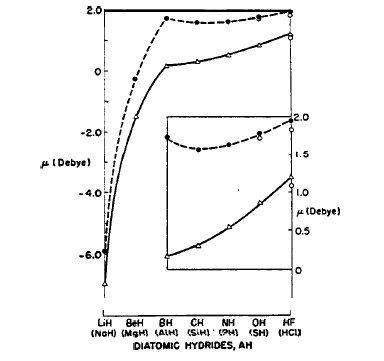
\includegraphics[width=0.6\textwidth]{images/mulliken_figure10.png}
\end{center}
%\captionsetup[figure]{labelsep=none}
\caption*{Figure 10: The dipole moment for the ground state of the first and second-row hydrides; first-row calculated values ($\bullet$), second-row calculated values (A), and experimental values ($\circ$).  Right-hand scale for small inset figure and left-hand scale for large figure.  Reproduced by permission of the authors (P.E. Cade and W.M. Huo, \emph{J. Chem. Phys.}45 (1966) 1063.)}
%\vspace{-10pt}
\end{figure}

\begin{figure}
\begin{center}
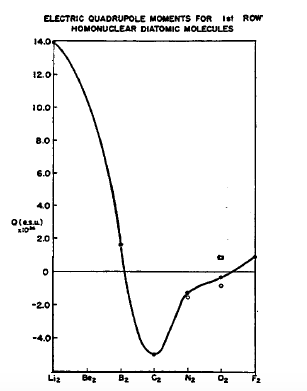
\includegraphics[width=0.5\textwidth]{images/mulliken_figure11.png}
\end{center}
%\captionsetup[figure]{labelsep=none}
\caption*{Figure 11: Reproduced by permission of Dr. Paul E. Cade, from unpublished work.}
%\vspace{-10pt}
\end{figure}



Figure 11 shows quadrupole moments of first-row homopolar diatomic molecules and radicals, as computed (Cade, unpublished) from accurate SCF-MO wave functions obtained by several investigators (Cade, Wahl, Malli, K. D. Sales and J. B. Greenshields) at Chicago by the use of the second machine program.  Here the sign of the quadrupole moment is sometimes positive, sometimes negative, and until recently was not known experimentally in any case. In Figure 11, the black circles are the computed values and the white circles are recent experimental values: for $\mathrm{N_2}$ by A. D. Buckingham, for $\mathrm{O_2}$ by microwave work, with sign uncertain; however, recently Buckingham has obtained an experimental value for $\mathrm{O_2}$ which on the scale of the curve is coincident with the computed value.

%insert Figure 12.
\begin{figure}
\begin{center}
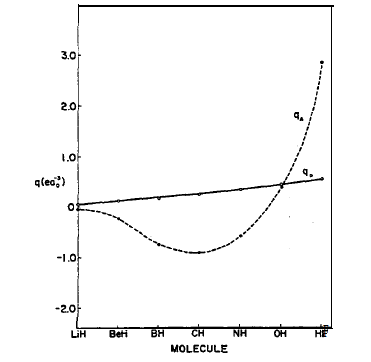
\includegraphics[width=0.5\textwidth]{images/mulliken_figure12.png}
\end{center}
%\captionsetup[figure]{labelsep=none}
\caption*{Figure 12: Electric field gradients, q, at A and H (or D) nuclei for first-row hydrides.  Reproduced from a forthcoming paper by P.E. Cade and W. Huo by permission of the authors; all rights reserved.}
%\vspace{-10pt}
\end{figure}

Figure 12 shows computed electric field gradients (nuclear quadrupole coupling constants) at the A and H (or D) nuclei in the first-row hydride molecules and radicals (from a forthcoming paper by Cade and Huo).  Here experimental data are available for $q_D$ in LiD and HD, but only indirectly from measured eqQ values and the nuclear quadrupole moment of the Deuteron, from accurate measurement and calculations on HD or $\mathrm{D_2}$.

Having accurate SCF-wave functions with spectroscopic MO's, one can ask, how well do these answer the questions with which chemists are concerned?  I have already referred to dipole moments and quadrupole moments, where agreement with true values is within 5 or $10\%$ in the examples where comparison was possible.\footnote{Of course an agreement in terms of \emph{percentage} is no longer relevant in cases where the value of the quantity is near zero.}  A similar degree of agreement is found for ionization potentials.  Moreover, all the ionization potentials which correspond to removal of a single electron from any outer or inner shell can be computed.  In all these cases we are dealing with properties that depend on one electron at a time.  For such cases there is a theorem which states that values computed from accurate SCF wave functions should be correct to first order.

But how about binding energies (dissociation energies) of molecules?  These are of very special interest to chemists.  Here we can subtract the SCF energy (the calculated energy of the SCF molecular wave function) from the sum of the SCF energies of the component atoms, and one might think that the difference should be the dissociation energy.  However, the agreements are generally poor; the calculated dissociation energies are often only half as large as they should be, or occasionally even come out less than zero.

There is a good reason for these disagreements, namely the fact that the electron-correlation energy of which I have spoken earlier is generally larger in a molecule than in the corresponding atoms.  In fact, as Clementi has pointed out, there is a more or less standard \emph{extra correlation energy} in a molecule for each chemical bond that is formed.  To deal with these need corrections to the SCF-computed dissociation energies, we can use empirical estimates, but a better way is also now in prospect.  Namely, instead of being satisfied with a SCF-wave function, which corresponds to a definite \emph{electron configuration}, that is, one definite assignment of electrons to MO's as in the Aufbauprinzip, we can go further by mixing into the wave function suitable amounts of wave functions corresponding to other judiciously chosen electron configurations.  In this way Das and Wahl\footnote{For some simple diatomic examples, see G. Das and A.C. Wahl, \emph{J. Chem. Phys.}, 44 (1966), 87.} at Chicago have made progress toward obtaining good theoretically calculated dissociation energies, and Clementi and others are pushing this work farther.

All the work on molecules so far described has been on diatomic molecules.  But most of chemistry is concerned with much larger molecules, with which McLean and Clementi made some all-electron LC$\cdot$STF approximate SCF-MO calculations on carbon dioxide, acetylene, cyanogen, hydrogen cyanide, and a number of other molecules.

Recently several groups have been using linear combinations of a different type of basis functions, namely Gaussian functions, instead of STF's, to build up approximate SCF-MO's.  For comparable accuracy, at least twice as many Gaussians as STF's must be used.  This procedure was first proposed by S. F. Boys of Cambridge, England.  Although Gaussians are intrinsically much poorer building blocks than STF's for constructing true MO's, calculations with them are easier, and it has proved possible to use them successfully to get rather good approximations to true SCF-MO wave functions.  Among those who have been using Gaussians recently are Moskowitz and Harrison using a machine program which was constructed by Harrison while working with Slater at M.I.T.; Allen and associates at Princeton; and recently Clementi, who spent most of the year 1966 at Chicago on leave from IBM's San Jos\'{e} Research Laboratory. 

During 1966 Clementi, with some cooperation of others, and with the use of copious amounts of machine time mostly at IBM's Yorktown laboratory, has carried through all-electron SCF-MO calculations of considerable accuracy on a notable array of molecules: ammonia, ethane, pyrrole, benzene, pyridine, and pyrazine.  Further, he has examined in detail what happens to MO's, to energies, and to charge distributions when a hydrogen chloride molecule approaches an ammonia molecule.

This last is of particular interest, but let me first mention the topic of population analysis.\footnote{R.S. Mulliken, \emph{J. Chem. Phys.}, 23 (1955) 1833-1840, 1841-1846, 2338-2342, 2343-2346.}  That technique makes it possible in a fairly meaningful way to calculate how the total population of electrons is distributed among the atoms in a molecules.  Among other things the procedure gives for each atom a number which can be identified as the electrical charge on that atom.  It also yields so-called \emph{overlap} populations, which are found to be well correlated with the strengths of chemical bonds.  I am sorry there is no time to explain the method here.  In a way it seems to contradict my basic theme that a molecule can better be thought of as an individual rather than a collection of atoms.  However, the molecule does contain atomic \emph{nuclei}, and the so-called charge on each atom in a molecule can be considered as an old-fashioned and familiar terminology for describing how electrical charge is distributed in the neighborhood of each nucleus.

The SCF-MO wave functions obtained at Chicago and elsewhere have yielded many interesting results when subjected to population analysis, but I will refer here only to one particularly interesting example, based on Clementi's calculation of what happens when an HCl approaches an $\mathrm{NH_3}$ molecule.  This case can be considered as an example of the formation of a molecular complex of a type which is particularly interesting, and is very important in biological systems, namely a hydrogen-bonded complex.  It has long been a moot question as to how the distribution of electrical charges changes during the approach of the two parters in a hydrogen-bonded complex.  Clementi's wave functions, when subjected to a population analysis, give an answer to this question, and his calculations also show how the energy changes during the approach.

What Clementi calculated were spectroscopic or true MO's for the combined \emph{system} $\mathrm{NH_3 + HCl}$.  This procedure, the whole-complex MO method, which could also be used with equal validity in understanding the electronic structure of any electron-donor electron-acceptor molecular complex,\footnote{Up to now I have used mainly a different procedure (R.S. Mulliken, \emph{J. Am. Chem. Soc.}, 74 (1952) 811; \emph{J. Chem. Phys.}, 60 (1964) 20) with a wave function corresponding partly or largely to an electron configuration of MO's of the free donor and acceptor, but with some mixing in of a second configuration in which an electron has been transferred from the donor to the acceptor.  For loose complexes the two procedures are roughly equivalent, but the whole-complex method is becoming advantageous now that all-electron SCF computations are becoming feasible for relatively large molecular systems.} represents another example of the improved understanding and accuracy which can result in going over from localized to delocalized MO's, -- in this case from MO's of the two molecules to MO's of the complex as a whole.

To justify the use of whole-complex MO's here, we note that each of the separate molecules $\mathrm{NH_3}$ and HCl has, in terms of MO's, a closed-shell electron configuration.  Now when two atoms in closed-shell AO configurations approach, for example, two helium atoms, the SCF-MO approximation remains a good approximation at all distances of approach.  In other words, there is then no large increase in electron correlation energy such as occurs when two atoms with unpaired valence electrons, for example two H atoms, or two N atoms, approach to form a molecule; it will be recalled that this increase in correlation energy on typical molecule formation had as a result that SCF-MO energies compared with SCF-AO energies do not give good values for dissociation energies.  By analogy with the case of two closed-shell atoms, it appears, however, that the SCF-MO approximation should be valid without any strongly varying electron correlation corrections when molecules with MO closed shells come together; the fact that two He atoms do not form a stable molecule does not matter for the present argument.  Thus Clementi's SCF-MO calculations on $\mathrm{NH_3 + HCl}$ should throw important light on the changes which occur in hydrogen bonding.  Actually, Clementi's calculations show a gradual transfer of charge from the $\mathrm{NH_3}$ to the Cl atom, accompanied by some stretching of the H-Cl distance, until at equilibrium a structure approaching that of an $\mathrm{NH_4^+ Cl^-}$ ion-pair, but with considerable polarization of the $\mathrm{Cl^-}$ (H-bonding of $\mathrm{NH_4}$ to $\mathrm{Cl^-}$) is attained.  The $\mathrm{NH_3 + HCl}$ system is thus apparently an example of ion-pair formation rather than ordinary loose hydrogen bonding; however, the changes in charge distribution during the early stages of approach of the HCl and $\mathrm{NH_3}$ should probably be similar to those in ordinary H-bonding, and thus instructive for the latter.

In conclusion, I would like to emphasize strongly my belief that the era of computing chemists, when hundreds if not thousands of chemists will go to the computing machine instead of the laboratory for increasingly many facets of chemical information\footnote{R.S. Mulliken and C.C.J. Roothann, ''Broken Bottlenecks and the Future of Molecular Quantum Mechanics,'' \emph{Proc. Natl. Acad. Sci. (U.S.)}, 45 (1959) 394-398.} is already at hand.  There is only one obstacle, namely that someone must pay for the computing time.  However, it seems clear that the provision of adequate funds by government and other organizations for computing molecular structures has at least as high an order of justification as the provision of adequate funds for the cyclotrons, betatrons, and linear accelerators used in studying nuclear structure and high-energy particles, or for rockets to explore the moon, planets, and interplanetary space.  Chemistry, together with physics of solid matter on the earth, deal with the foundations of the material world on which all our life is built. Yet at the present time the rapid progress which could be made even with existing machine programs is not being made, simply because available funds to pay for machine time are far too limited.  Computing time is rather expensive, yet the amounts of time needed to make adequate use of existing and future machine programs would be trivially small compared with the amount now being spent on nuclear and high-energy problems and on outer space.


\end{document}


%%% Local Variables:
%%% mode: latex
%%% TeX-master: t
%%% End:
